\documentclass{article}

\usepackage{graphicx} % Required for inserting images
\usepackage{tikz} % Pack para fazer as representações de figuras
\usepackage{listings}
\usepackage{xcolor}
\usepackage{amsfonts}
\usepackage{float}
\usepackage{amsmath}
\usepackage{authblk}
% \usepackage{geometry}

\usepackage[margin=2.5cm]{geometry}
\usepackage{hyperref}
\hypersetup{
    colorlinks=true,
    linkcolor=blue,
    urlcolor=blue,
    citecolor=blue,
}
\lstset{
    language=Python,
    basicstyle=\ttfamily\small,
    keywordstyle=\color{blue},
    commentstyle=\color{green!60!black},
    stringstyle=\color{red},
    numbers=left,
    numberstyle=\tiny\color{gray},
    frame=single,
    breaklines=true,
    showstringspaces=false
}


\title{Ciência de Redes}

\author{Henrique Borges Carvalho \hspace{35px} Raphaella Roma Mendes Alves}
% COlocar link pro repositório aqui
\date{
    November 2025 \\ 
    \href{https://github.com/SeuUsuario/SeuRepositorio}{Repositório}
}
\begin{document}

\maketitle

\section{SIS Model}

O Modelo SIS é um modelo epidemiológico que busca representar a propagação de um patógeno de maneira simples, onde os indivíduos são separados em dois grupos, sucetíveis e infectantes, e cada grupo é afetado de acordo com um parâmetro $\mu$ e $\beta$.

\begin{figure}[ht]
    \centering
    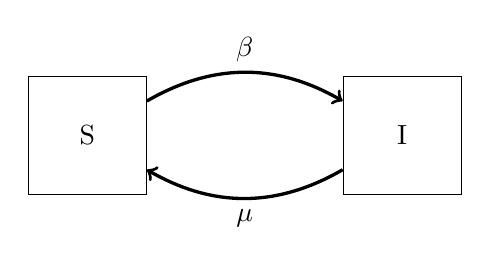
\begin{tikzpicture}
        [
        state/.style={rectangle, draw, minimum size=1.5cm} 
        ]

        \node[state] (S) at (0,0) {S};
        \node[state] (I) at (4,0) {I};

        \draw[->, very thick, bend left=30] (S) to node[midway, above] {$\beta$} (I);
        \draw[->, very thick, bend left=30] (I) to node[midway, below] {$\mu$} (S);
    
    \end{tikzpicture}
    \caption{SIS Model}
    \label{SIS Model}
\end{figure}

Aqui $\beta$ é a probabilidade de um indivíduo sucetível se tornar infectado no contato com um vizinho infectado e $\mu$ é a probabilidade de um indivíduo infectado se tornar sucetível.

Vamos calcular a quantidade de infectados no tempo $T$ junto a taxa de variação de indivíduos infectados. A partir da equação de diferenças:
\[
I_{t+1} = I_t - I_t\mu + \left( \langle k\rangle \frac{I_t}{N}\beta   \right) (N-I_t)
\]
De fato, se tenho $I_t$ infectados no tempo $t$, para encontrar a quantidade de infectados no tempo $t+1$ tenho de considerar quantos dos indivíduos infectados se tornam sucetíveis, o que é expresso por $I_t\mu$, e também quantos sucetíveis se tornam infectados, expresso por $\left( \langle k\rangle \frac{I_t}{N}\beta   \right) (N-I_t)$, onde $N-I_t$ é a quantidade de sucetíveis e seguindo a hipótese de \textbf{mistura homogênea} temos $\langle k\rangle \frac{I_t}{N}\beta $ para a probabilidade de um sucetível se tornar infectado.
\[
\Delta I_t =  I_{t+1} - I_t = - I_t\mu + \left( \langle k\rangle \frac{I_t}{N}\beta   \right) (N-I_t)
\]
\[
\Delta \frac{I_t}{N} = -\frac{I_t}{N}\mu + \left( \langle k\rangle \frac{I_t}{N}\beta   \right) \left(1 - \frac{I_t}{N}\right)
\]
Assumindo estado estacionário temos:
\[
0 = -\frac{I_t}{N}\mu + \left( \langle k\rangle \frac{I_t}{N}\beta   \right) \left(1 - \frac{I_t}{N}\right) = \frac{I_t}{N}\left( -\mu +  \left( \langle k\rangle \beta  \right) \left( 1 - \frac{I_t}{N}\right) \right)
\]
Essa equação tem duas soluções, uma onde $\frac{I_t}{N} = 0$, caso trivial e a outra onde:
\[
-\mu +  \left( \langle k\rangle \beta  \right) \left( 1 - \frac{I_t}{N}\right)  = 0
\]
Que nos leva a:
\[
\mu = \langle k \rangle \beta - \langle k \rangle \beta \frac{I_t}{N} \Rightarrow \frac{I_t}{N} = 1  - \frac{\mu}{\langle k \rangle \beta} 
\]
Portanto:
\[
\frac{I_t}{N} = 1 - \frac{1}{R_0}
\]
E chegamos as conclusões que se $R_0$ é maior do que $1$ então a doença se fixa na rede pois $\frac{I_t}{N} > 0$. Se $R_0 <= 1$, então $\frac{I_t}{N} \leq 0$ e a doença tende a sumir da rede.

\section{Experimentos em redes Erdos-Renyi}
Gere uma rede aleatória (ER) com 10000 vértices e grau médio $\langle k \rangle = 20$. Comece com 5 vértices infectados escolhidos aleatoriamente. Execute múltiplas simulações da propagação da infecção pelo modelo SIS com os parâmetros abaixo e compare com os resultados esperados. (sugestão: faça em torno de 100 simulações e descreva o comportamento da epidemia ``na média'')

\begin{enumerate}
    \item[(a)] $\beta = 0.02$ e $\mu = 0.1$
    \item[(b)] $\beta = 0.02$ e $\mu = 0.4$
    \item[(c)] $\beta = 0.02$ e $\mu = 0.5$
\end{enumerate}

Mostre que se $R_0 = \frac{\beta \langle k \rangle}{\mu} > 1$ então a doença se fixa na rede no modelo SIS de campo médio.

\subsection{Gerando rede}
Utilizando o pacote \textbf{networkx} do python podemos obter um rede aleatória passando os parâmetros $n$ e $p$ que são respectivamente a quantidade de nós e a probabilidade de existir uma aresta entre dois nós. Assim para obtermos uma rede aleatória com grau médio $<k> = 20$ precisamos encontrar $p$.

Sabemos que a soma dos graus do nós em uma rede não direcionada é duas vezes a quantidade de arestas

\[
\sum_i^n k_i = 2E = 2 \left( p \frac{n(n-1)}{2} \right)
\]

Logo:
\[
\mathbb{E} \left(\sum_i^n k_i\right) = \sum_i^n\mathbb{E}(k_i)= n<k> = pn(n-1)  = \mathbb{E}  \left(2 p \frac{n(n-1)}{2} \right)
\]

Portanto $p = \frac{<k>}{n-1}$.

No nosso caso temos $n = 10.000$ e $<k> = 20 $ resultando em $p = \frac{20}{10.000 - 1}$

Portanto podemos obter a rede da seguinte forma:

\begin{lstlisting}
import networkx as nx

n = 10000
k_medio = 20

# Probabilidade de conexao para rede ER
p = k_medio / (n - 1)

G_ER = nx.erdos_renyi_graph(n, p)

\end{lstlisting}

Gerando a rede podemos plotar a sua distribuição dos graus:

\begin{figure}[H]
    \centering
    \includegraphics[width=0.8\linewidth]{figures/q1/Q1_distribuicao_graus.png}
    \caption{Distribuição dos graus de G\_ER}
    % \label{fig:placeholder}
\end{figure}

Como esperado, segue uma distribuição normal com média em 20.

\subsection{item (a)}
O item (a) pede os seguintes valores para $\beta$ e $\mu$:
\[
\beta = 0.02 \qquad \mu = 0.1 
\]
calculando obtemos $R_0 = 20 \frac{0.02}{0.1} = 4 $ e como vimos anteriormente, $R_0  > 1$ resulta em uma fixação da doença na rede.

Realizando o experimento computacional de 100 simulações de 100 estados de tempo obtemos o seguinte:

\begin{figure}[H]
    \centering
    \includegraphics[width=0.8\linewidth]{figures/q1/Q1a_simulacoes.png}
    \caption{Simulação: $R_0 > 1 $}
    % \label{fig:placeholder}
\end{figure}

Como vemos no gráfico, a doença se fixa na rede convergindo próximo a fração estacionária $\frac{I_t}{N} = 1 - \frac{1}{R_0} = 0.75$.

\subsection{item (b)}
O item (b) pede os seguintes valores para $\beta$ e $\mu$:

\[
\beta = 0.02 \qquad \mu = 0.4 
\]

calculando obtemos $R_0 = 20 \frac{0.02}{0.4} = 1 $. Aqui temos $R_0 \leq 1$, o que significa que a doença tende a sumir da rede, entretanto $R_0$ é exatamente 1, o que nos coloca em uma espécie de \textit{estado crítico} onde comportamentos inesperados podem acontecer.

Realizando o experimento computacional de 100 simulações de 100 estados de tempo podemos observar alguns desses comportamentos inesperados:

\begin{figure}[H]
    \centering
    \includegraphics[width=0.8\linewidth]{figures/q1/Q1b_simulacoes.png}
    \caption{Simulação: $R_0 = 1$}
    % \label{fig:placeholder}
\end{figure}

Vemos que na média, a quantidade de infectados se mantém constante, entretanto há uma grande variação na quantidade de infectados nas simulações indo de $0$ a $60$. Concluimos pela média constante na quantidade de infectados inicialmente e pelo decaimento dos percentis $25$-$75$ que mesmo em estado crítico, a doença não domina a rede, se apresentando similar a uma epidemia.

\subsection{item (c)}
O item (c) pede os seguintes valores para $\beta$ e $\mu$:
\[
\beta = 0.02 \qquad \mu = 0.5 
\]
Aqui nos deparamos com $R_0 = 20\frac{0.02}{0.5} = 0.8 < 1 $, portanto esperamos um comportamento onde a doença se estingue na rede, fazendo as simulações temos o seguinte:

\begin{figure}[H]
    \centering
    \includegraphics[width=01\linewidth]{figures/q1/Q1c_simulacoes.png}
    \caption{Simulação: $R_0 < 1$}
    % \label{fig:placeholder}
\end{figure}

Aqui fica evidente o resultado esperado, a doença se estingue na rede tendo poucos casos de grandes flutuações.

\section{Experimentos em redes de livre escala}
Gere uma rede livre de escala com 10000 vértices, grau médio $\langle k \rangle = 20$ e expoente $\gamma = 2.5$. Comece com 5 vértices infectados escolhidos aleatoriamente. Execute múltiplas simulações da propagação da infecção pelo modelo SIS com os parâmetros abaixo e compare com os resultados esperados. (sugestão: faça em torno de 100 simulações e descreva o comportamento da epidemia ``na média'')

\begin{enumerate}
    \item[(a)] $\beta = 0.01$ e $\mu = 0.1$
    \item[(b)] $\beta = 0.01$ e $\mu = 0.2$
    \item[(c)] $\beta = 0.01$ e $\mu = 0.3$
\end{enumerate}

Descreva o comportamento da epidemia e compare com o item (1).

\subsection{Gerando a rede}

Utilizando o pacote \textbf{networkx} do Python, podemos gerar uma rede livre de escala a partir de uma sequência de graus que obedece à lei de potência
\[
P(k)\propto k^{-\gamma},
\]
onde $\gamma$ é o expoente e $k$ é o grau do nó. Para controlar simultaneamente o expoente $\gamma$ e o grau médio alvo $\langle k\rangle$, adotamos o \emph{modelo de configuração} com algumas precauções práticas.

\subsubsection{Modelo de Configuração --- passos}

\textbf{1. Geração da sequência de graus} \\
Geramos $n$ amostras da distribuição de potência por transformada inversa. Com $r\sim\mathcal{U}(0,1)$:
\[
k = \Big(k_{\min}^{\,1-\gamma} + r\,(k_{\max}^{\,1-\gamma}-k_{\min}^{\,1-\gamma})\Big)^{\frac{1}{1-\gamma}},
\]
onde $k_{\min}\ge 1$ e $k_{\max}= n-1$ (permitindo que qualquer nó possa, 
em princípio, conectar-se a todos os demais; cutoffs adicionais como 
$k_{\max}=n^{1/(\gamma-1)}$ são opcionais mas podem reduzir flutuações 
em redes pequenas).

\vspace{5px}
\textbf{2. Ajuste do grau médio} \\
Calcule a média da sequência gerada e aplique um fator multiplicativo:
\[
\text{fator}=\frac{\langle k\rangle_{\text{alvo}}}{\langle k\rangle_{\text{atual}}},\qquad
k_i'=\max(1,\;\lfloor k_i\cdot\text{fator}\rfloor).
\]
Usar arredondamento/clip para manter $1\le k_i'\le n-1$.

\vspace{5pt}
\textbf{3. Garantia de soma par e validade gráfica} 

Assegure que $\sum_i k_i'$ é par (se for ímpar, incremente um grau arbitrário). Verifique também se a sequência é \emph{graphical} (teste de Erdős–Gallai / networkx.is\_graphical). Se não for, aplique pequenas perturbações randômicas e reavalie; se falhar, considere regenerar.

\vspace{4px}
\textbf{4. Construção do grafo simples} \\
Recomenda-se usar \texttt{nx.havel\_hakimi\_graph(seq)} para obter um grafo simples que reproduza a sequência exata de graus (sem loops nem múltiplas arestas). Como alternativa, é possível usar \texttt{nx.configuration\_model(seq)} e depois converter para grafo simples removendo loops/múltiplas arestas, mas note que essa limpeza altera a sequência de graus e, portanto, pode mudar $\langle k\rangle$ e a cauda da distribuição — deve ser reportado.

\subsubsection{Implementação (exemplo)}

\begin{lstlisting}
def gerar_rede_scale_free(n, k_medio_alvo, gamma, max_tentativas=50, seed=42):
    np.random.seed(seed)
    k_min = max(1, int(max(2, k_medio_alvo // 4)))
    k_max = n - 1
    melhor_G = None
    melhor_diff = float('inf')
    for tentativa in range(max_tentativas): # Amostragem por transformada inversa
        u = np.random.random(n)
        if gamma == 1:
            ks = k_min * (k_max / k_min) ** u
        else:
            a = k_min ** (1 - gamma)
            b = k_max ** (1 - gamma)
            ks = (a + u * (b - a)) ** (1.0 / (1 - gamma))
        seq = np.maximum(1, np.floor(ks)).astype(int).tolist()
        media = np.mean(seq)  # Ajusta para grau medio alvo
        fator = k_medio_alvo / media
        seq = np.clip(np.round(np.array(seq)*fator).astype(int), 1,n-1).tolist()
        if sum(seq) % 2 == 1: # Garante soma par
            idx = np.random.randint(0, n)
            seq[idx] = min(n - 1, seq[idx] + 1)
        if nx.is_graphical(seq): # Tenta construir grafo simples
            G = nx.havel_hakimi_graph(seq)
            if nx.is_connected(G):
                k_real = np.mean([d for _, d in G.degree()])
                diff = abs(k_real - k_medio_alvo)
                if diff < 1.0:
                    return G
                if diff < melhor_diff:
                    melhor_diff = diff
                    melhor_G = G
    
    return melhor_G  # Retorna melhor rede encontrada
\end{lstlisting}

Ao gerar uma rede desse modo com os parâmetros desejados obtemos o seguinte gráfico da distribuição de grau dos nós 

\begin{figure}[H]
    \centering
    \includegraphics[width=0.8\linewidth]{figures/q2/Q2_distribuicao_graus.png}
    \caption{Distribuição dos graus: Livre de escala}
    \label{fig:placeholder}
\end{figure}
\subsubsection{Verificação do Expoente}

Após gerar a rede, é importante verificar se o expoente $\gamma$ da distribuição 
gerada está próximo ao valor desejado. Para isso, utilizamos a Complementary 
Cumulative Distribution Function (CCDF):

\[
\text{CCDF}(k) = P(K \ge k) = \sum_{k'=k}^{k_{\max}} P(k')
\]

Se $P(k) \sim k^{-\gamma}$, então $\text{CCDF}(k) \sim k^{-(\gamma-1)}$.

Em um gráfico log-log de CCDF vs. $k$, temos:
\[
\log(\text{CCDF}(k)) = -(\gamma-1) \log(k) + c
\]

Ajustando uma reta por regressão linear, obtemos:
\[
\gamma_{\text{estimado}} = -\text{slope} + 1
\]

O coeficiente de determinação $R^2$ indica a qualidade do ajuste à lei de potência.

Para nossa rede gerada, obtivemos:
\begin{itemize}
    \item $\gamma_{\text{estimado}} = 2.58$ (próximo ao alvo $\gamma = 2.5$)
    \item $R^2 = 0.997$ (ajuste excelente)
\end{itemize}

\subsection{Item (a)}
O primeiro experimento utiliza os parâmetros:
\[
\beta = 0.01 \qquad \mu = 0.1
\]
Calculando o $R_0 = 20 \frac{0.01}{0.1} = 2$ imaginamos que pela análise feita nas seções anteriores, a doença deve se estabelecer na rede.

Fizemos um experimento computacional, agora com 1000 passos, justamente para verificar se existem padrões mais interessantes nas redes livres de escala. 
\begin{figure}[H]
    \centering
    \includegraphics[width=0.8\linewidth]{figures/q2/Q2a_simulacoes.png}
    \caption{Simulação: 2 (a)}
    % \label{fig:placeholder}
\end{figure}

Podemos ver que a variancia em cada simulação é ampla, mas seguindo pela média há evidente uma tendência da doença se estabelecer, abaixo temos alguns resultados mais detalhados 
\begin{lstlisting}
Resultados (100 simulacoes):
  Infectados no estado estacionario: 879.76 +- 841.03
  Epidemias extintas: 43/100 (43.0%)
\end{lstlisting}
Aqui conseguimos entender um pouco melhor o gráfico acima, estranhamente, quase metade das simulações a doença se estingue, o que não era o esperado dado que $R_0 > 1$. Isso se justifica pois em redes livres de escala não é válido assumir a hipótese de \textbf{mistura homogênea}. Vamos prosseguir com os experimentos e no final da seção veremos mais sobre o SIS sem assumir tal hipótese.

\subsection{Item (b)}
Já essa experimento utiliza os parâmetros:
\[
\beta = 0.01 \qquad \mu = 0.2
\]
Vamos novamente calcular o $R_0 = 20 \frac{0.01}{0.2} = 1 $. Segundo o modelo de campo médio, esperariamos que a doença não apresentasse comportamento similar ao que vimos em (1.b).

Segue o experimento computacional:

\begin{figure}[H]
    \centering
    \includegraphics[width=0.8\linewidth]{figures/q2/Q2b_simulacoes.png}
    \caption{Simulação: 2 (b)}
    % \label{fig:placeholder}
\end{figure}

Novamente vemos um comportamento fora do esperado em comparação ao que já vimos, entretanto ao menos a fixação na rede parece ter reduzido em magnitude de pessoas em comparação com o que vimos para $R_0 = 2$.

\begin{lstlisting}
Resultados (100 simulacoes):
  Infectados no estado estacionario: 254.14 +- 379.60
  Epidemias extintas: 69/100 (69.0%)
\end{lstlisting}

Vemos que em boa parte das simulações a doença não se fixa na rede, entretanto nosso $R_0$ é bem próximo de 1 o que nos levaria a crer que a doença deveria se estinguir em todos os casos.

\subsection{Item (c)}
Por fim, esse experimento utiliza os parâmetros:
\[
\beta = 0.01 \qquad \mu = 0.3
\]
Agora o nosso $R_0 \approx 0.67$ nos leva a crer que a doença será extinta da rede, entretanto não é o que vemos na simulação:

\begin{figure}[H]
    \centering
    \includegraphics[width=0.8\linewidth]{figures/q2/Q2c_simulacoes.png}
    \caption{Simulação: 2(c)}
    % \label{fig:placeholder}
\end{figure}

Esse é um dos casos mais interessantes pois a doença se fixa na rede, em alguns casos com uma quantidade de pessoas relativamente alta, mas na média ficamos com algo em torno de 150 pessoas.
\begin{lstlisting}
Resultados (100 simulacoes):
  Infectados no estado estacionario: 141.67 +- 245.68
  Epidemias extintas: 75/100 (75.0%)
\end{lstlisting}
Vendo os resultados mais questionamentos são levantados, mas é inegável que redes aleatórias tem resultados muito distintos de redes livres de escala (ao menos no nosso caso onde $\gamma = 2.5$) de modo que não podemos avaliar tais discrepâncias como meras flutuações probabilisticas.

\subsection{Modelo SIS em redes heterogêneas}

Nos itens anteriores, observamos que os resultados experimentais divergem significativamente das previsões do modelo de campo médio. Em particular, no item (c) vimos que mesmo com $R_0 = 0.67 < 1$, a doença consegue se fixar na rede em 25\% das simulações, contradizendo a teoria que desenvolvemos na primeira seção.

A questão que surge naturalmente é: \textit{o que está errado na nossa análise?}

A resposta está na hipótese de \textbf{mistura homogênea} que assumimos ao derivar o modelo de campo médio. Essa hipótese pressupõe que todos os indivíduos têm a mesma probabilidade de interagir entre si, o que é equivalente a assumir que todos os nós têm aproximadamente o mesmo grau. Isso é razoável para redes Erdős-Rényi, onde a distribuição de graus é aproximadamente Poisson e concentrada em torno de $\langle k \rangle$. Entretanto, em redes livres de escala, a distribuição de graus segue uma lei de potência $P(k) \sim k^{-\gamma}$, o que implica em uma \textit{heterogeneidade} extrema: temos tanto nós com pouquíssimas conexões quanto \textit{hubs} com centenas ou milhares de conexões.

\subsubsection{O problema com o $R_0$ de campo médio}

Vamos relembrar como chegamos na expressão para o $R_0$ de campo médio. Partimos da equação:
\[
\Delta I_t = -I_t\mu + \left( \langle k\rangle \frac{I_t}{N}\beta   \right) (N-I_t)
\]

O termo $\langle k\rangle \frac{I_t}{N}\beta$ representa a probabilidade de um suscetível se infectar. Implicitamente, estamos assumindo que cada suscetível tem $\langle k \rangle$ vizinhos e que a probabilidade de um vizinho estar infectado é $\frac{I_t}{N}$ (mistura homogênea).

Em redes heterogêneas, essa aproximação falha por dois motivos:

\begin{enumerate}
    \item Nós com graus diferentes têm probabilidades diferentes de se infectar
    \item Nós com graus diferentes contribuem de forma diferente para a propagação
\end{enumerate}

Em particular, os \textit{hubs} (nós com $k \gg \langle k \rangle$) têm um papel desproporcional na dinâmica epidêmica. Um hub infectado pode infectar dezenas ou centenas de vizinhos, enquanto um hub suscetível tem alta probabilidade de se infectar pois está conectado a muitos nós.

\subsubsection{Limiar epidêmico em redes heterogêneas}

Para corrigir o modelo, precisamos levar em conta a distribuição de graus. Pastor-Satorras e Vespignani (2001) mostraram que, para redes heterogêneas, o limiar epidêmico crítico é dado por:

\[
R_0^{\text{crítico}} = \frac{\langle k \rangle}{\langle k^2 \rangle}
\]

onde $\langle k^2 \rangle = \sum_k k^2 P(k)$ é o segundo momento da distribuição de graus.

Comparando com o limiar de campo médio ($R_0^{\text{crítico}} = 1$), vemos que o novo limiar depende da \textit{variância} da distribuição de graus. Para redes com distribuição homogênea (como ER), temos $\langle k^2 \rangle \approx \langle k \rangle^2$, o que recupera $R_0^{\text{crítico}} \approx 1$. Entretanto, para redes scale-free com $\gamma \le 3$, o segundo momento $\langle k^2 \rangle$ pode ser extremamente grande (ou até divergir no limite $N \to \infty$), fazendo com que $R_0^{\text{crítico}} \to 0$.

Isso tem uma implicação surpreendente: \textbf{em redes scale-free, praticamente qualquer doença, por mais fraca que seja, pode se tornar endêmica}.

\subsubsection{Aplicando a teoria à nossa rede}

Vamos calcular $R_0^{\text{crítico}}$ para a rede que geramos. Nossa rede tem:

\begin{lstlisting}
Estatisticas da rede:
  <k> (grau medio):           20.16
  <k^2> (segundo momento):    2406.87
  k_max (grau maximo):        1713
\end{lstlisting}

Portanto:
\[
R_0^{\text{crítico}} = \frac{20.16}{2406.87} \approx 0.0084
\]

Esse valor é \textbf{muito menor que 1}! Vamos agora reanalisar nossos três experimentos à luz dessa nova teoria:

\begin{table}[H]
\centering
\begin{tabular}{|c|c|c|c|c|}
\hline
\textbf{Item} & $\boldsymbol{R_0}$ (campo médio) & $\boldsymbol{R_0 > R_0^c}$? & \textbf{Previsão} & \textbf{Observado} \\
\hline
(a) & 2.02 & Sim (2.02 $>>$ 0.0084) & Endêmica & 57\% persistentes \\
(b) & 1.01 & Sim (1.01 $>>$ 0.0084) & Endêmica & 31\% persistentes \\
(c) & 0.67 & Sim (0.67 $>>$ 0.0084) & Endêmica & 25\% persistentes \\
\hline
\end{tabular}
\caption{Comparação entre previsões e resultados observados}
\end{table}

Vemos que \textbf{todos os três cenários} satisfazem $R_0 > R_0^{\text{crítico}}$ e, portanto, todos deveriam apresentar comportamento endêmico segundo a teoria de redes heterogêneas. Isso está em concordância com nossas observações: mesmo no item (c), onde o campo médio previa extinção, vimos que 25\% das epidemias persistiram.

\subsubsection{Por que algumas epidemias ainda se extinguem?}

Se todos os cenários são endêmicos segundo a teoria, por que observamos taxas de extinção de 43\%, 69\% e 75\% nos itens (a), (b) e (c), respectivamente?

A teoria de Pastor-Satorras e Vespignani é derivada no limite termodinâmico ($N \to \infty$) e assume tempo infinito. Na prática, estamos lidando com uma rede finita ($N = 10000$) e tempo finito (1000 passos), o que introduz efeitos estocásticos importantes:

\begin{enumerate}
    \item \textbf{Condições iniciais}: Começamos com apenas 5 infectados escolhidos aleatoriamente. Se esses infectados iniciais estiverem em regiões periféricas da rede (longe dos hubs), a epidemia pode se extinguir antes de atingir os hubs.
    
    \item \textbf{Flutuações estocásticas}: Mesmo em um cenário endêmico, flutuações aleatórias podem levar à extinção, especialmente quando o número de infectados é baixo. Quanto menor o $R_0$, maior a probabilidade dessas flutuações causarem extinção.
    
    \item \textbf{Tempo finito}: Para valores de $R_0$ próximos ao limiar crítico (como no item c), o sistema pode levar muito tempo para convergir ao estado estacionário endêmico. Em 1000 passos, algumas epidemias podem ainda estar em processo de crescimento lento.
\end{enumerate}

Isso explica por que a taxa de extinção aumenta de (a) para (c): embora todos sejam endêmicos em teoria, quanto menor o $R_0$, mais próximo estamos do limiar e mais suscetível o sistema está a flutuações que levam à extinção.

\subsubsection{Comparação com redes Erdős-Rényi}

Para finalizar, vamos comparar os resultados das redes ER (questão 1) com as redes scale-free (questão 2). Embora tenhamos usado $\beta$ diferentes nos dois casos, podemos comparar cenários com $R_0$ similares:

\begin{itemize}
    \item \textbf{Rede ER com $R_0 = 1$}: A epidemia apresentou comportamento crítico, com alta variabilidade mas tendência de extinção na maioria dos casos.
    
    \item \textbf{Rede scale-free com $R_0 = 1.01$}: A epidemia persiste em 31\% dos casos, significativamente mais que o esperado para campo médio.
    
    \item \textbf{Rede scale-free com $R_0 = 0.67$}: Mesmo abaixo do limiar de campo médio, a epidemia persiste em 25\% dos casos.
\end{itemize}

A diferença fundamental está na \textit{heterogeneidade}. Em redes ER, todos os nós são aproximadamente equivalentes, e o limiar $R_0 = 1$ é bem definido. Em redes scale-free, os hubs criam "super-espalhadores" que mantêm a epidemia viva mesmo em condições que, segundo campo médio, deveriam levar à extinção.

\section{Estratégias de Imunização}

Nessa seção vamos estudar diferentes estratégias de imunização na rede livre de escala gerada na questão anterior. O objetivo é descobrir qual a fração mínima de nós que precisam ser imunizados previamente para impedir a fixação do estado endêmico.

Utilizaremos os parâmetros do item (a) da questão 2: $\beta = 0.01$ e $\mu = 0.1$, que resultam em $R_0 = 2.02$. Esse valor alto de $R_0$ indica uma epidemia forte, o que significa que será necessária uma fração significativa de imunizados para suprimir a doença.

\subsection{Estratégias de imunização}

Vamos comparar três estratégias diferentes:

\begin{enumerate}
    \item \textbf{Imunização Aleatória}: Escolhe nós aleatoriamente para imunizar. Essa é a estratégia mais simples, mas também a menos eficiente em redes heterogêneas.
    
    \item \textbf{Imunização de Hubs}: Escolhe os nós com maior grau (os hubs) para imunizar. Essa estratégia explora a estrutura da rede, removendo os nós mais conectados.
    
    \item \textbf{Imunização de Vizinhos (Acquaintance Immunization)}: Escolhe nós aleatórios e imuniza seus vizinhos. Essa estratégia se baseia no "paradoxo da amizade": em média, seus amigos têm mais amigos que você. Logo, escolher vizinhos de nós aleatórios tende a selecionar nós mais conectados, sem necessitar conhecimento completo da rede.
\end{enumerate}

\subsection{Metodologia}

Para cada estratégia, testamos diferentes frações de imunização (de 0\% a 70\% dos nós) e executamos múltiplas simulações. Consideramos que a epidemia foi controlada quando menos de 10\% das simulações apresentam comportamento endêmico.

\subsection{Resultados}

Realizando os experimentos computacionais obtemos o seguinte gráfico comparativo:

\begin{figure}[H]
    \centering
    \includegraphics[width=0.8\linewidth]{figures/q3/Q3_comparacao_estrategias.png}
    \caption{Comparação de estratégias de imunização em rede scale-free}
    \label{fig:q3_comparacao}
\end{figure}

Podemos observar alguns padrões interessantes no gráfico acima:

\begin{itemize}
    \item \textbf{Estratégia de Hubs (vermelho)}: É claramente a mais eficiente. A curva cai rapidamente, alcançando o limiar de 10\% de epidemias persistentes com aproximadamente 36\% dos nós imunizados.
    
    \item \textbf{Estratégia Aleatória (azul)}: É a menos eficiente. A curva cai lentamente e não alcança o limiar de 10\% mesmo com 50\% dos nós imunizados, necessitando de frações ainda maiores.
    
    \item \textbf{Estratégia de Vizinhos (verde)}: Apresenta eficiência intermediária entre hubs e aleatória, mas nesse caso específico com $R_0$ alto, também não alcançou o limiar com 50\% de imunização.
\end{itemize}

\subsection{Discussão: Por que imunizar hubs é tão eficiente?}

A grande diferença de eficiência entre as estratégias pode ser explicada pela estrutura heterogênea da rede scale-free. Vamos entender o que acontece em cada caso:

\subsubsection{Imunização Aleatória}

Quando imunizamos nós aleatoriamente em uma rede scale-free, estamos removendo principalmente nós de grau baixo, já que eles são a maioria. Entretanto, os hubs permanecem intactos e continuam atuando como super-espalhadores. É necessário imunizar uma fração muito alta da população até que, por acaso, comecemos a atingir os hubs.

Matematicamente, a probabilidade de escolher um hub aleatoriamente é proporcional à sua frequência na rede. Como hubs são raros em redes scale-free (seguem $P(k) \sim k^{-\gamma}$), a imunização aleatória demora muito para atingi-los.

\subsubsection{Imunização de Hubs}

Ao imunizar diretamente os hubs, estamos removendo os nós que:
\begin{enumerate}
    \item Têm alta probabilidade de se infectar (pois estão conectados a muitos outros nós)
    \item Podem infectar muitos vizinhos se ficarem doentes
    \item Conectam diferentes partes da rede (têm alta centralidade)
\end{enumerate}

Removendo os hubs, a rede se fragmenta rapidamente. O que antes era uma grande componente conexa se quebra em várias componentes menores, dificultando a propagação global da epidemia.

Esse comportamento está relacionado com a robustez de redes scale-free: são robustas a falhas aleatórias (remoção aleatória afeta pouco) mas vulneráveis a ataques direcionados (remoção de hubs fragmenta rapidamente).

\subsubsection{Imunização de Vizinhos}

A estratégia de vizinhos explora o paradoxo da amizade. Em redes, a distribuição de graus dos vizinhos de um nó tende a ter média maior que a distribuição geral de graus. Isso acontece porque nós com grau alto aparecem como vizinhos de mais nós.

Formalmente, se $P(k)$ é a distribuição de graus, a distribuição de graus dos vizinhos é proporcional a $kP(k)$. Para nossa rede scale-free com $P(k) \sim k^{-2.5}$, temos que os vizinhos seguem $k \cdot k^{-2.5} = k^{-1.5}$, uma distribuição com cauda ainda mais pesada.

Portanto, escolher vizinhos de nós aleatórios tende a selecionar nós mais conectados que a média, sendo mais eficiente que imunização aleatória pura.

\subsection{Fração crítica de imunização}

Com base nos resultados obtidos, podemos estimar a fração crítica $f_c$ necessária para controlar a epidemia:

\begin{table}[H]
\centering
\begin{tabular}{|l|c|c|}
\hline
\textbf{Estratégia} & \textbf{Fração Crítica} & \textbf{Nós Imunizados} \\
\hline
Hubs & $\sim$36\% & $\sim$3600 nós \\
Vizinhos & $>$50\% & $>$5000 nós \\
Aleatória & $>$50\% & $>$5000 nós \\
\hline
\end{tabular}
\caption{Fração crítica de imunização para cada estratégia}
\end{table}

Vemos que imunizar hubs é aproximadamente 1.4x mais eficiente que imunização aleatória. Essa diferença pode parecer modesta, mas em uma população de 10000 indivíduos, representa economizar mais de 1400 doses de vacina.

\subsection{Relação com $R_0$ heterogêneo}

É interessante notar que mesmo com uma fração alta de imunização aleatória, a epidemia persiste. Isso reforça o que vimos na seção anterior sobre o limiar epidêmico em redes heterogêneas.

Quando imunizamos uma fração $f$ da população aleatoriamente, o grau médio efetivo da rede diminui para $\langle k \rangle_{\text{ef}} = (1-f)\langle k \rangle$. Entretanto, o segundo momento $\langle k^2 \rangle$ não diminui proporcionalmente, pois os hubs (que contribuem enormemente para $\langle k^2 \rangle$) têm baixa probabilidade de serem removidos.

Assim, o limiar crítico:
\[
R_0^{\text{crítico}} = \frac{\langle k \rangle_{\text{ef}}}{\langle k^2 \rangle_{\text{ef}}}
\]

permanece muito baixo mesmo com imunização aleatória, exigindo frações muito altas de imunização.

Em contraste, quando imunizamos hubs, reduzimos drasticamente $\langle k^2 \rangle$, pois estamos removendo exatamente os nós que mais contribuem para esse momento. Isso eleva rapidamente o limiar crítico, tornando a rede menos suscetível a epidemias.

\subsection{Implicações práticas}

Esses resultados têm implicações diretas para políticas de saúde pública:

\begin{enumerate}
    \item \textbf{Vacinação prioritária}: Em situações de escassez de vacinas, priorizar indivíduos com muitos contatos sociais (professores, profissionais de saúde, trabalhadores de transporte público) é muito mais eficiente que vacinação aleatória.
    
    \item \textbf{Identificação de super-espalhadores}: Investir em identificar e monitorar indivíduos altamente conectados pode ser crucial para controle epidêmico.
    
    \item \textbf{Acquaintance immunization}: Quando não há informação completa sobre a rede de contatos, a estratégia de vizinhos oferece um meio-termo: é mais eficiente que aleatória sem exigir mapeamento completo da rede.
    
    \item \textbf{Vulnerabilidade de redes reais}: Muitas redes reais (contatos sociais, transporte aéreo, comércio internacional) têm características scale-free. Isso as torna especialmente vulneráveis a epidemias, mesmo com $R_0$ relativamente baixo segundo campo médio.
\end{enumerate}

\subsection{Observação sobre $R_0$ alto}

Vale notar que utilizamos $R_0 = 2.02$, um valor relativamente alto que representa uma epidemia forte. Por isso, mesmo a estratégia mais eficiente (hubs) requer imunizar mais de 1/3 da população. Para doenças com $R_0$ menor, as frações críticas seriam significativamente menores, mas a hierarquia de eficiência entre as estratégias se manteria: hubs > vizinhos > aleatória.

\section{Conclusão}

Neste trabalho estudamos a propagação de epidemias usando o modelo SIS em diferentes topologias de rede. Os resultados demonstraram que a estrutura da rede é tão importante quanto os parâmetros epidemiológicos para determinar o destino de uma epidemia.

Em redes Erdős-Rényi (homogêneas), o modelo de campo médio se mostrou válido: o limiar epidêmico $R_0 = 1$ foi confirmado pelas simulações. Entretanto, em redes livres de escala (heterogêneas), observamos comportamento drasticamente diferente. Mesmo com $R_0 = 0.67 < 1$, 25\% das epidemias persistiram, contradizendo as previsões de campo médio.

A explicação está nos \textit{hubs}: nós extremamente conectados que atuam como super-espalhadores. Nossa rede scale-free apresentou um limiar epidêmico real de $R_0^{\text{crítico}} \approx 0.0084$, muito menor que 1, devido ao segundo momento $\langle k^2 \rangle = 2406.87$ causado pelos hubs. Isso significa que praticamente qualquer doença pode se tornar endêmica em redes heterogêneas.

As estratégias de imunização confirmaram a importância dos hubs: vacinar os nós mais conectados requer apenas $\sim$36\% de cobertura, enquanto vacinação aleatória precisa de $>$50\%, economizando mais de 1400 doses em uma população de 10000 indivíduos.

A principal lição é clara: \textbf{políticas de controle epidêmico devem considerar a topologia da rede}. Modelos de campo médio podem subestimar drasticamente o risco de pandemias em redes reais (que frequentemente são heterogêneas), e estratégias de vacinação direcionada aos indivíduos altamente conectados são muito mais eficientes. 

\end{document}
